%%%%%%%%%%%%%%%%%%%%%%%%%%%%%%%%%%%%%%%%%
% Facial Expresion Recognition with Convolutional Neural Networks
% 
% Lewe Ohlsen
% Fachhochschule Wedel
%
% Latex Template by Frits Wenneker (http://www.howtotex.com)
%
%%%%%%%%%%%%%%%%%%%%%%%%%%%%%%%%%%%%%%%%%

%----------------------------------------------------------------------------------------
%	PACKAGES AND OTHER DOCUMENT CONFIGURATIONS
%----------------------------------------------------------------------------------------

\documentclass[twoside]{article}

\usepackage{lipsum} % Package to generate dummy text throughout this template
\usepackage{graphicx} % Figures from matplotlib
\graphicspath{ {figures/} }

\usepackage[sc]{mathpazo} % Use the Palatino font
\usepackage[T1]{fontenc} % Use 8-bit encoding that has 256 glyphs
\linespread{1.05} % Line spacing - Palatino needs more space between lines
\usepackage{microtype} % Slightly tweak font spacing for aesthetics

\usepackage[hmarginratio=1:1,top=32mm,columnsep=20pt]{geometry} % Document margins
\usepackage{multicol} % Used for the two-column layout of the document
\usepackage[hang, small,labelfont=bf,up,textfont=it,up]{caption} % Custom captions under/above floats in tables or figures

\usepackage{booktabs} % Horizontal rules in tables
\usepackage{float} % Required for tables and figures in the multi-column environment - they need to be placed in specific locations with the [H] (e.g. \begin{table}[H])
\usepackage{hyperref} % For hyperlinks in the PDF

\usepackage{paralist} % Used for the compactitem environment which makes bullet points with less space between them

\usepackage{abstract} % Allows abstract customization
\renewcommand{\abstractnamefont}{\normalfont\bfseries} % Set the "Abstract" text to bold
\renewcommand{\abstracttextfont}{\normalfont\small\itshape} % Set the abstract itself to small italic text

\usepackage{titlesec} % Allows customization of titles
\usepackage[utf8]{inputenc}
%\renewcommand\thesection{\Roman{section}} % Roman numerals for the sections
%\renewcommand\thesubsection{\Roman{subsection}} % Roman numerals for subsections
\titleformat{\section}[block]{\large\scshape\centering\bfseries}{\thesection.}{1em}{} % Change the look of the section titles
\titleformat{\subsection}[block]{}{\thesubsection.}{1em}{} % Change the look of the section titles


%----------------------------------------------------------------------------------------
%	TITLE SECTION
%----------------------------------------------------------------------------------------

\title{\vspace{-15mm}\fontsize{16pt}{10pt}\selectfont\textbf{Facial Expression Recognition with\\ Convolutional Neural Networks}} % Article title 

\author{
	\large
	\textsc{Lewe Ohlsen}\\[2mm] % Your name
	\normalsize Fachhochschule Wedel \\ % Your institution
	\normalsize \href{mailto:minf101062@fh-wedel.de}{minf101062@fh-wedel.de} % Your email address
	\vspace{-5mm}
}
\date{}

%----------------------------------------------------------------------------------------

\begin{document}

\maketitle % Insert title

%----------------------------------------------------------------------------------------
%	ABSTRACT
%----------------------------------------------------------------------------------------

\begin{abstract}

\noindent El barómetro es un instrumento de medición atmosérica, específicamente utilizado en la determinación de la fuerza por unidad de superficie ejercida por el peso de la atmósfera. Existe un gran número de equipos atmoféricos con distintos tipos de estos aparátos y son diariamente utilizados ya que la presión atmosférica juega un papel importante en la determinación y pronóstico del tiempo así como en el área de investigación al momento de realizarse experimentos ya que pueden llegar a afectar o hacer variar el funcionamiento de muchos aparatos electrónicos y mecánicos.

\end{abstract}

%----------------------------------------------------------------------------------------
%	ARTICLE CONTENTS
%----------------------------------------------------------------------------------------

\begin{multicols}{2} % Two-column layout throughout the main article text

\section{Introduction}

Automatically recognizing facial expressions is an interesting and challenging problem in many fields, including human computer interaction (HCI) and artificial emotional intelligence. This projects goal is to develop a classifier for real-time detection of facial expressions. 

As Convolutional Neural Networks (CNNs) have proven to be successful with many kinds of image classification  problems, I will focus on building a classifier using a state of the art CNN implementation.

%------------------------------------------------

\section{Datasets}

Paul Ekmans 1969 research paper "Facial Expressions" (REF) elaborates that facial expressions can be interpreted and categorized into six classes of basic emotion that can be found across all human cultures: anger, disgust, fear, happiness, sadness, and surprise. In this project, these classes are used for training and predictions.

To build a classifier for facial expressions, a dataset with labeled images of faces is required. Each of the datasets is split into two subsets: A training set that is used to fit the prediction and a test set to evaluate the prediction results.

\subsection{FER-2013}

The FER-2013 Dataset consists of roughly 37.000 images showing faces of people expressing a certain emotion. Most of the 48x48 pixel grayscale images are stock footage. These images have been centered on the persons faces to show a similar region in every sample. As this has been done automatically, some images are not centered correctly. Faces are depicted from very different angles, hence generalization of these samples is difficult. 

\begin{figure}[H]
	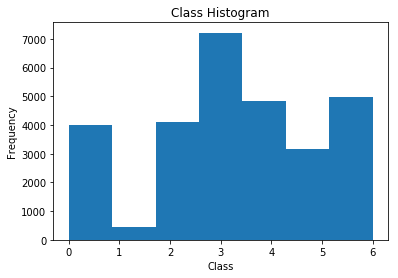
\includegraphics[width=0.48\textwidth]{class_dist}
	\caption{FER-2013 emotion class distribution}
\end{figure}

The class labels were crowd-sourced with Amazon Mechanical Turk, where quality work is not incentivised, so we can expect label-noise to be significant. It is expected that every subject shows only a single emotion, where in reality faces can express mixed emotions (e.g happiness and surprise). A research group at Microsoft (who?) decided to minimize label-noise in FER-2013 by re-labeling the dataset (REF). Ten workers on MTurk were asked to label each image, yielding a probability distribution of emotion classes instead of a single class for each image.




\subsection{Cohn-Kanade (CK+)}
To augument the wild variety of FER-2013 images, a second, more conservative dataset with only frontal faces is considered. The Cohn-Kanade (CK+) dataset consists of 593 image sequences across 123 subjects. Each image sequence goes from a neutral facial expression to a "peak expression" according to the six basic emotions. Only 327 of the 593 image sequences are labeled with emotion data. This is because not all images fit the prototypic definition of the Facial Action Coding System (FACS) according to Ekman et al. CK+ also contains FACS data, in which facial action units (e.g raised eyebrow) are identified along with their degree of activation.

Figure of CK+ distribution with neutral images.

%------------------------------------------------

\section{Related work}


%------------------------------------------------

\section{Discussion and Conclusion}



%----------------------------------------------------------------------------------------
%	REFERENCE LIST
%----------------------------------------------------------------------------------------

\begin{thebibliography}{9}

	% OpenCV Haarcascade Classifier
	\bibitem{violajones}
  	P. A. Viola and M. J. Jones. Robust real-time face detection.
	International Journal of Computer Vision
	57(2):137–154, 2004.

	% the ICML 2013 workshop’s facial expression recognition challenge
	\bibitem{replearning}
	I. J. Goodfellow et al.
	Challenges in representation learning: A report on three machine
	learning contests.
	Neural Networks
	, 64:59 – 63, 2015.
	Special Issue on ‘Deep Learning of Representations’

 
\end{thebibliography}

%----------------------------------------------------------------------------------------

\end{multicols}

\end{document}
